% report.tex for DA project

\documentclass{article}
\usepackage[utf8]{inputenc}
\usepackage{graphicx}
%\usepackage{placeins}

\begin{document}

\begin{center}
\LARGE
\textbf{Abstract}
\end{center}

\normalsize
This report is an analysis of a 120 hour period at the Conway, Arkansas airport that looks at temperature and dew point to determine the likelihood of fog formation. Thes author uses a Python program to input data in the form of a '.txt' file. The data are aviation weather reports that contain, among other items, the temperature and dew point . These reports, issued at an hourly minimum, are the actual reports generated, either, automatically or by weather observers, for aviators to determine current weather conditions. When the spread is less than 2 degrees Celsius, the likelihood is that fog may form.

\bigskip
\begin{flushleft}
\textbf{keywords:} temperature, dew point
\end{flushleft}

\newpage


\title{Conway, Arkansas Airport - Temperature/Dew Point Analysis}
\author{John Singel}\date{May 11, 2021}

\maketitle

\section{Introduction}
In aviation there is an old saying: 'An excellent pilot is one who uses his excellent brain so that he does not have to use his excellent skills.' For over a century, now, aviators have relied on mnemonics and other devices to recall important information in a timely manner. These devices span from systems knowledge to preflight planning. One handy weather tool is the knowledge that when the temperature and dew point difference is two degrees Celsius or less, the chance of fog forming is high. This knowledge, in turn, will spur the aviator to plan for alternates and contingencies.

\section{METAR/Weather}
METAR stands for Meterological Aerodrome Forecast. It is a standard format used to promulgate aviation weather information. A standard METAR is shown below:
\medskip
\begin{center}
KCXW 101350Z AUTO 05008KT 10SM OVC020 12/08 A3008 RMK A01
\end{center}
\medskip
The first block is the four letter identifier for the specific airport, in this case Conway's Cantrell Field. The second block is the date/time group. The first two numbers are the day of the month and the last four are the time, in Zulu, or Universal Time Coordinated (UTC), of the observations. The third block tells the type of observation, in this case automated. The fourth block contains the wind direction in relation to true north and the speed (here, from the northeast, 050 degrees, at 8 knots). The fifth block is the visibility in statute miles. The sixth block is the current cloud conditions. Here the observation tells us that it is overcast and the clouds are at 2,000 above the ground. The seventh block contains the temperature and dew point separated by a slash, in degrees Celsius. The eighth block is the barometric pressure, or altimeter setting. The ninth block contains the remarks, which in this case, tell us what type of automated weather reporting we have (A01). 

\section{Analysis}

\begin{figure}[h]
\begin{center}
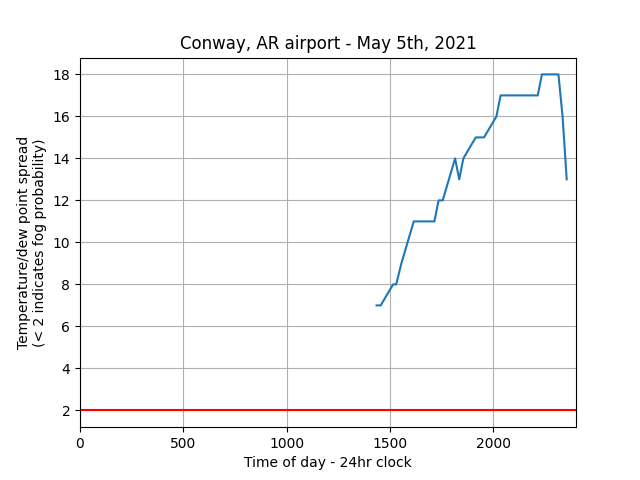
\includegraphics[width=1\textwidth]{May5th.png}
\end{center}
\caption{May 5th temperature/dew point spread}
\label{May 5th}
\end{figure}

\begin{figure}[h]
\begin{center}
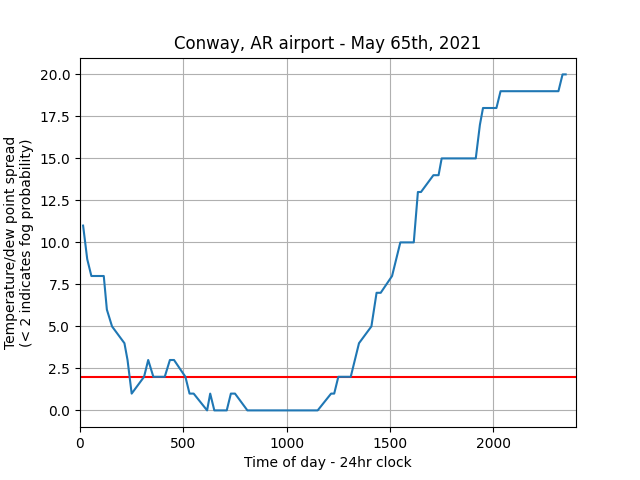
\includegraphics[width=1\textwidth]{May6th.png}
\end{center}
\caption{May 6th temperature/dew point spread}
\label{May 6th}
\end{figure}

\begin{figure}[h]
\begin{center}
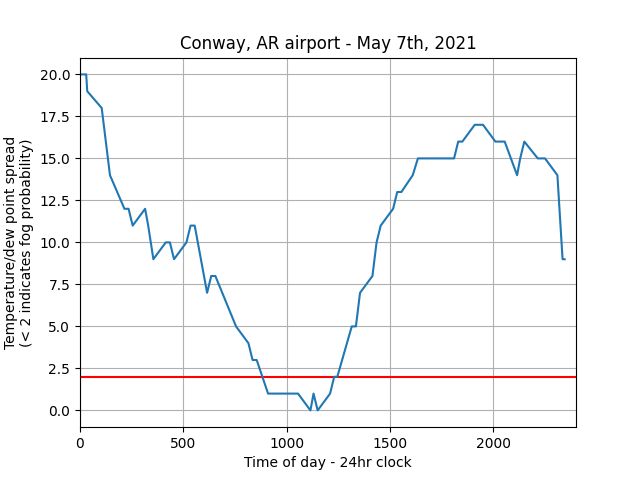
\includegraphics[width=1\textwidth]{May7th.png}
\end{center}
\caption{May 7th temperature/dew point spread}
\label{May 7th}
\end{figure}

\begin{figure}[h]
\begin{center}
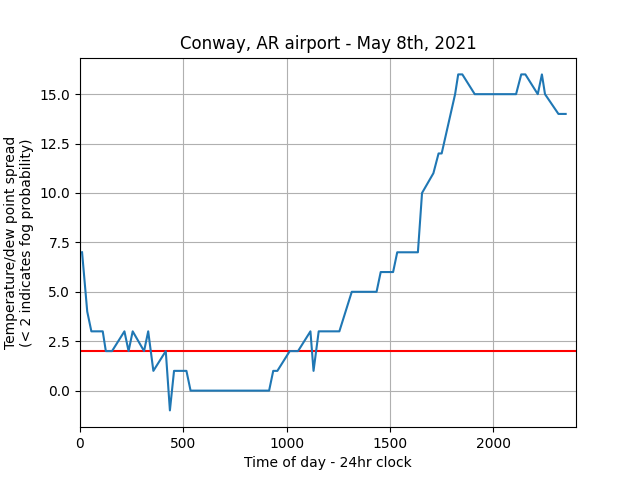
\includegraphics[width=1\textwidth]{May8th.png}
\end{center}
\caption{May 8th temperature/dew point spread}
\label{May 8th}
\end{figure}

\begin{figure}[h]
\begin{center}
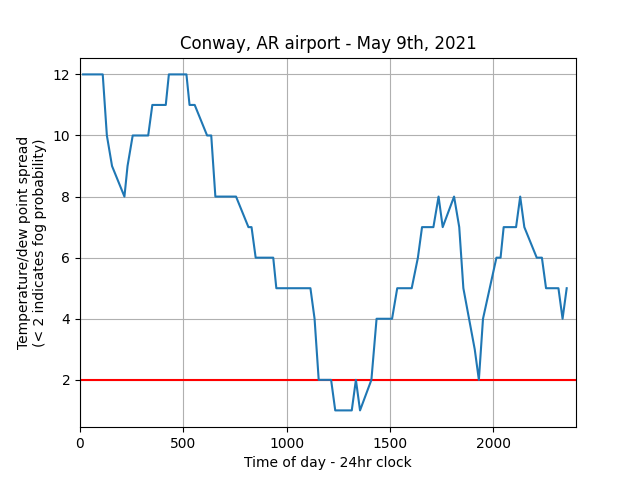
\includegraphics[width=0.5\textwidth]{May9th.png}
\end{center}
\caption{May 9th temperature/dew point spread}
\label{May 9th}
\end{figure}

\begin{figure}[h]
\begin{center}
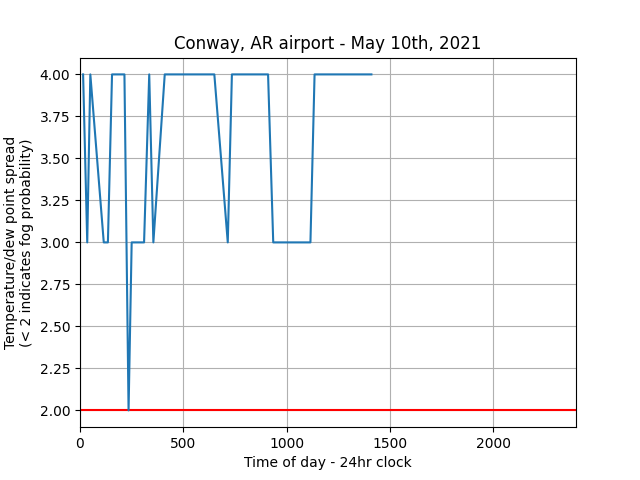
\includegraphics[width=1\textwidth]{May10th.png}
\end{center}
\caption{May 10th temperature/dew point spread}
\label{May 10th}
\end{figure}

%\FloatBarrier

\section{Conclusion}

\subsection{How to use labels}
When referring to an item previously lableled, use the name of the label. For example: Figure  \ref{May 6th}

$\alpha\lambda\lambda  \Gamma\rho\epsilon\epsilon\kappa$

\end{document}

